% Provenance (never printed): cycle 4 SVT/physique, "La planete Terre,
% l'environnement": the movements of the atmosphere, weather and its
% forecast; see sources/book1/PROVENANCE.md. Book 1, grade 8, chapter 3.
% Vocabulary guard: owns air mass, front (warm, cold), depression (homograph:
% phrase-level linking only), anticyclone, isobar, weather forecast. The
% rotation of the winds around lows and highs is told (deflection, recalled
% from ch. g8.2); the occluded front is named in prose only; numerical models
% are told, not taught.
\chapter{Air Masses, Fronts and Weather Maps}\label{ch:g8:fronts-and-weather-maps}

The morning is bright and still. Around noon, thin white streaks appear
very high in the sky, and slowly spread into a pale veil that dims the
Sun. In the afternoon the \omterm{def:g4:clouds-rain-snow:cloud}{clouds} thicken and come lower; by evening a
steady \omterm{def:g4:clouds-rain-snow:precipitation}{rain} is falling. During the night it turns warm and damp, then a
dark line of \omterm{def:g4:clouds-rain-snow:cloud}{cloud} brings a short burst of heavy \omterm{def:g4:clouds-rain-snow:precipitation}{rain} and a gust of wind.
The next morning is clear, fresh and windy. In two days a
\emph{\omterm{def:g8:fronts-and-weather-maps:depression}{depression}} has passed over the town, with its two \omterm{def:g8:fronts-and-weather-maps:front}{fronts}.
% ledger: ucar:warm-front, ucar:cold-front

\begin{omfigure}
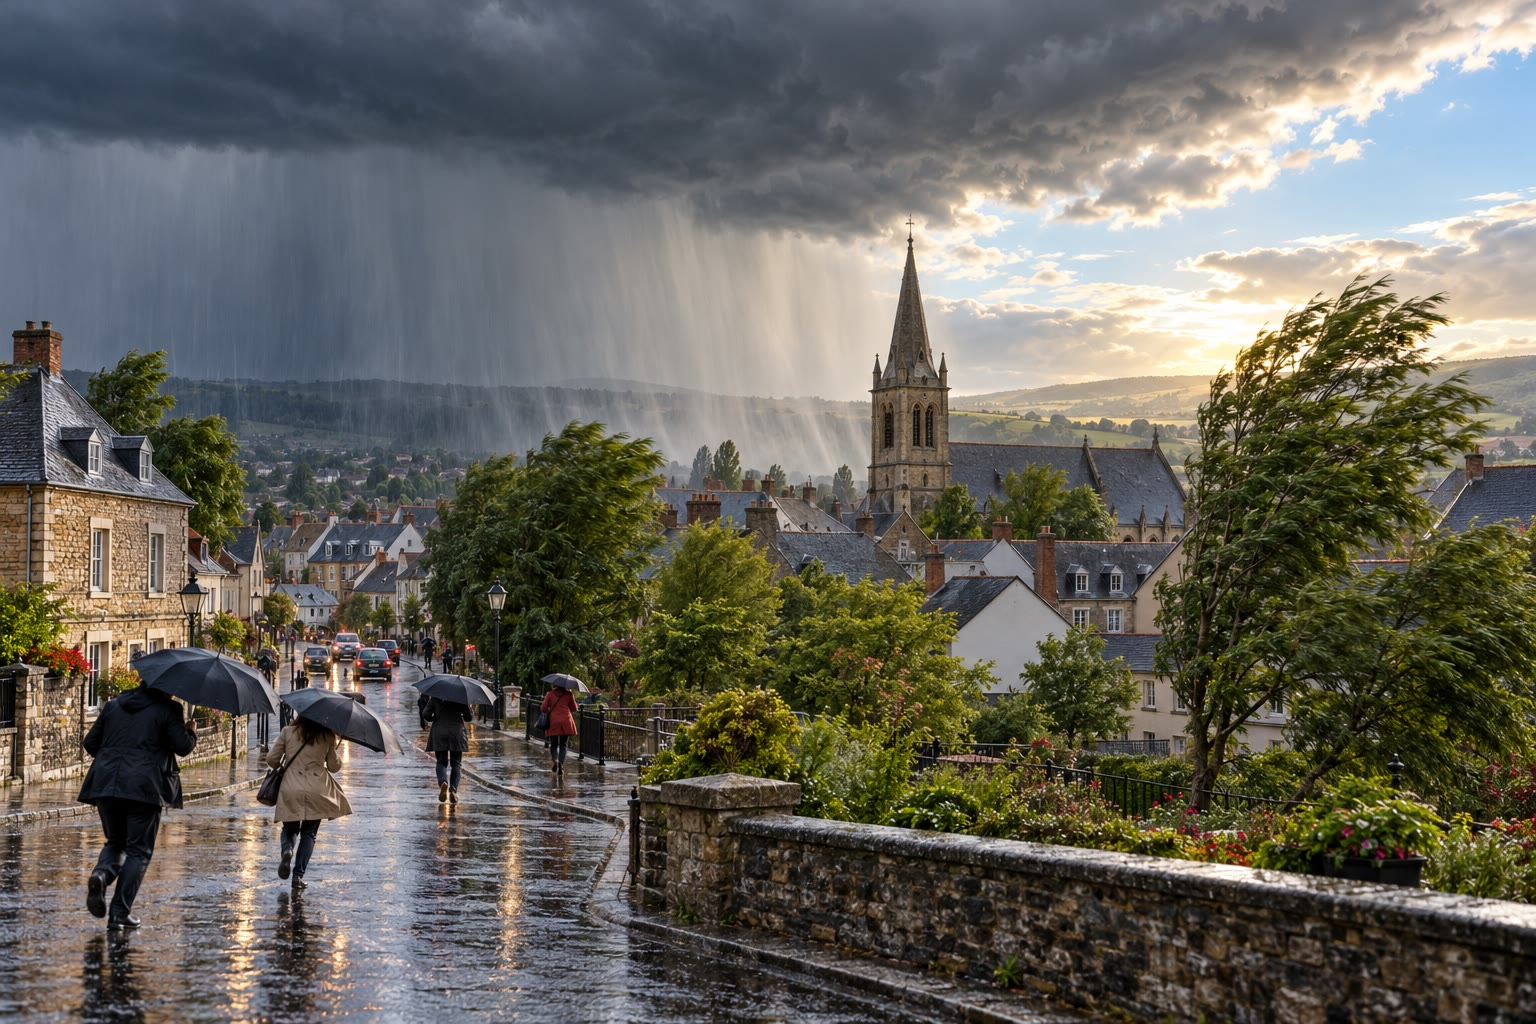
\includegraphics[width=0.6\linewidth]{images/book1/ai/g8-rain-arriving.jpg}

{\small A curtain of \omterm{def:g4:clouds-rain-snow:precipitation}{rain} arrives over a town under a dark \omterm{def:g4:clouds-rain-snow:cloud}{cloud} base,
while the sky is still clear behind the church (AI-generated illustration
of a generic scene).}
\label{fig:g8:fronts-and-weather-maps:rain}
\end{omfigure}

\omterm{def:g1:watching-the-weather:weather}{Weather} forecasters saw it coming days before. This chapter shows how:
the air of our skies comes in large masses, the masses meet along
\omterm{def:g8:fronts-and-weather-maps:front}{fronts}, and \omterm{def:g2:drawing-to-map:map}{maps} of the pressure show where they are going.

\begin{recall}
Air presses on everything it touches; a barometer measures this pressure
in hectopascals (the physics books), and at \omterm{def:g4:world-physical-map:altitude}{sea level} it is about
\qty{1013}{hPa} (\cref{ch:g8:the-atmosphere}). \omterm{def:g4:clouds-rain-snow:cloud}{Clouds} form when damp air
rises and cools (\cref{ch:g4:clouds-rain-snow}). At the ground, the wind
blows from high pressure towards low pressure, and the Earth's rotation
turns it aside: to the right in the \omterm{def:g3:continents-and-oceans:equator}{northern hemisphere}. Between about
\ang{30} and \ang{60}, the \omterm{def:g8:winds-global-circulation:global-winds}{westerlies} bring one \omterm{def:g5:natural-hazards:storm}{storm} after another
(\cref{ch:g8:winds-global-circulation}).
\end{recall}

\section{Air masses}

Air that stays for days over the same place takes on the character of
the surface beneath it. Over a warm \omterm{def:g2:water-on-earth:ocean}{ocean} it becomes warm and damp; over a
frozen land, cold and dry. When it moves away, it carries this character
with it, sometimes for thousands of kilometres.
% ledger: noaa:air-mass

\begin{definition}[Air mass]\label{def:g8:fronts-and-weather-maps:air-mass}
An \emph{air mass}\index{air mass} is a very large body of air in which
the temperature and the humidity are nearly the same everywhere at a
given height. It takes them from the region where it formed, its
\emph{source region}.
\end{definition}
% ledger: noaa:air-mass

Forecasters name an \omterm{def:g8:fronts-and-weather-maps:air-mass}{air mass} with two letters. The first says where it
formed: \emph{c} (continental) over land, so it is dry; \emph{m}
(maritime) over an \omterm{def:g2:water-on-earth:ocean}{ocean}, so it is moist. The second says how cold it
is: \emph{A} (arctic) over the polar regions, \emph{P} (polar) over the
high \omterm{def:g6:latitude-longitude:latitude}{latitudes}, \emph{T} (tropical) over the low \omterm{def:g6:latitude-longitude:latitude}{latitudes}. Air from a
hot \omterm{def:g5:weather-and-climate:desert}{desert} is cT, hot and dry; air from the Arctic is cA, very cold and
dry.
% ledger: noaa:air-mass

\begin{omfigure}
\begin{tikzpicture}
\begin{axis}[ommap, width=12.6cm, xmin=-100, xmax=60, ymin=10, ymax=85,
  xtick={-90,-60,...,60}, ytick={20,40,60,80},
  xticklabels={$90^\circ$W,$60^\circ$W,$30^\circ$W,$0^\circ$,$30^\circ$E,$60^\circ$E},
  yticklabels={$20^\circ$N,$40^\circ$N,$60^\circ$N,$80^\circ$N},
  tick label style={font=\scriptsize}]
  \addplot[fill=omLithAlluv, draw=black!45, line width=0.2pt] table {figdata/out/shared-geo-land.dat};
  \tikzset{src/.style={line width=0.9pt, fill opacity=0.35, text opacity=1, font=\scriptsize, align=center}}
  \draw[src, draw=omCold, fill=omCold!35] (axis cs:-30,79) ellipse [x radius=26, y radius=4.5];
  \node[font=\scriptsize, align=center, fill=white, inner sep=1pt] at (axis cs:-30,79) {\textbf{cA}: very cold, dry};
  \draw[src, draw=omCold, fill=omCold!25] (axis cs:-35,55) ellipse [x radius=14, y radius=6];
  \node[font=\scriptsize, align=center, fill=white, inner sep=1pt] at (axis cs:-35,55) {\textbf{mP}: cold,\\ moist};
  \draw[src, draw=omCold, fill=omCold!25] (axis cs:-84,60) ellipse [x radius=12, y radius=7];
  \node[font=\scriptsize, align=center, fill=white, inner sep=1pt] at (axis cs:-84,60) {\textbf{cP}: cold,\\ dry};
  \draw[src, draw=omCold, fill=omCold!25] (axis cs:45,62) ellipse [x radius=14, y radius=7];
  \node[font=\scriptsize, align=center, fill=white, inner sep=1pt] at (axis cs:45,62) {\textbf{cP}: cold,\\ dry};
  \draw[src, draw=omWarm, fill=omWarm!25] (axis cs:-45,28) ellipse [x radius=16, y radius=6];
  \node[font=\scriptsize, align=center, fill=white, inner sep=1pt] at (axis cs:-45,28) {\textbf{mT}: warm,\\ moist};
  \draw[src, draw=omWarm, fill=omWarm!25] (axis cs:10,24) ellipse [x radius=15, y radius=6];
  \node[font=\scriptsize, align=center, fill=white, inner sep=1pt] at (axis cs:10,24) {\textbf{cT}: hot,\\ dry};
\end{axis}
\end{tikzpicture}

{\small Typical source regions of air masses around the North Atlantic
(schematic): over the Arctic, the cold \omterm{def:g3:continents-and-oceans:continent}{continents}, the northern \omterm{def:g2:water-on-earth:ocean}{ocean}, the
subtropical \omterm{def:g2:water-on-earth:ocean}{ocean} and the Sahara. Blue: cold air masses; red: warm ones.}
% ledger: noaa:air-mass, data:ne-land (schematic regions)
\label{fig:g8:fronts-and-weather-maps:sources}
\end{omfigure}

\section{Fronts}

When an \omterm{def:g8:fronts-and-weather-maps:air-mass}{air mass} moves, it meets another one. The two do not mix
easily: they stay apart, with a narrow boundary between them where the
\omterm{def:g1:watching-the-weather:weather}{weather} changes.
% ledger: mo:fronts, ucar:cold-front

\begin{definition}[Front]\label{def:g8:fronts-and-weather-maps:front}
A \emph{front}\index{front} is the boundary at the ground between two air
masses of different temperature and humidity. At a \emph{cold
front}\index{cold front}, cold air pushes into warmer air and takes its
place; at a \emph{warm front}\index{warm front}, warm air pushes into
colder air and takes its place.
\end{definition}
% ledger: mo:fronts, ucar:cold-front, ucar:warm-front

Cold air is denser than warm air. At a \omterm{def:g8:fronts-and-weather-maps:front}{cold front}, the cold air slides
under the warm air like a wedge and lifts it up sharply. The warm, damp air
rises fast and builds towering \omterm{def:g4:clouds-rain-snow:cloud}{clouds}, \omterm{def:g4:clouds-rain-snow:cloud-families}{cumulus} and \omterm{def:g4:clouds-rain-snow:cloud-families}{cumulonimbus}: the \omterm{def:g8:fronts-and-weather-maps:front}{front}
brings heavy showers, sometimes \omterm{def:g4:clouds-rain-snow:precipitation}{hail} and thunder, gusts of wind and a
sudden drop in temperature. Once it has passed, the \omterm{def:g4:clouds-rain-snow:precipitation}{rain} stops and the sky
clears. A \omterm{def:g8:fronts-and-weather-maps:front}{cold front} moves fast, up to twice as fast as a \omterm{def:g8:fronts-and-weather-maps:front}{warm front}.
% ledger: ucar:cold-front

\begin{omfigure}
\begin{tikzpicture}[font=\footnotesize, >={Stealth[length=2.2mm]}, yscale=0.7, xscale=0.95]
  % ground
  \draw[line width=0.8pt] (0,0) -- (15,0);
  % cold wedge, nose at x = 8.2
  \fill[omCold!18] (0,0) -- (0,3.4) .. controls (4.5,3.2) and (7.2,2.4) .. (7.9,0.8)
    .. controls (8.1,0.35) and (8.2,0.12) .. (8.25,0) -- cycle;
  \draw[omCold, line width=1pt] (0,3.4) .. controls (4.5,3.2) and (7.2,2.4) .. (7.9,0.8)
    .. controls (8.1,0.35) and (8.2,0.12) .. (8.25,0);
  \node[omCold, align=center] at (3.2,1.4) {\textbf{cold air}\\(dense)};
  \node[omWarm, align=center] at (12.6,1.4) {\textbf{warm, damp air}};
  % cold air pushes
  \draw[->, omCold, line width=1.2pt] (4.6,0.5) -- (7.0,0.5);
  % warm air lifted
  \draw[->, omWarm, line width=1.2pt] (11.2,0.45) .. controls (9.4,0.6) and (8.6,1.4) .. (8.5,3.0);
  % cumulonimbus
  \fill[black!12] (7.3,2.6) .. controls (7.0,3.4) and (7.4,4.2) .. (7.9,4.5)
    .. controls (7.6,5.0) and (8.6,5.2) .. (9.4,5.1) -- (11.0,5.15)
    .. controls (10.6,4.9) and (10.2,4.8) .. (10.0,4.6)
    .. controls (10.4,4.0) and (10.2,3.0) .. (9.8,2.5) -- cycle;
  \draw[black!45] (7.3,2.6) .. controls (7.0,3.4) and (7.4,4.2) .. (7.9,4.5)
    .. controls (7.6,5.0) and (8.6,5.2) .. (9.4,5.1) -- (11.0,5.15)
    .. controls (10.6,4.9) and (10.2,4.8) .. (10.0,4.6)
    .. controls (10.4,4.0) and (10.2,3.0) .. (9.8,2.5) -- cycle;
  \node at (9.0,3.8) {cumulonimbus};
  \foreach \x in {7.7,8.0,...,9.6} \draw[omCold!70, line width=0.5pt] (\x,2.45) -- (\x-0.25,0.15);
  \node[anchor=west, align=left] at (9.8,1.95) {heavy showers,\\gusts};
  % motion
  \draw[->, line width=1.3pt] (5.7,4.3) -- (7.2,4.3);
  \node[anchor=east] at (5.6,4.3) {the front moves};
  \node[anchor=north] at (8.25,-0.1) {front at the ground};
  \node[anchor=north west, align=left] at (0.1,-0.1) {behind: cooler, clearing};
  \node[anchor=north east, align=right] at (15,-0.1) {ahead: warm, damp};
\end{tikzpicture}

{\small A \omterm{def:g8:fronts-and-weather-maps:front}{cold front} seen from the side (heights much exaggerated). The
cold air pushes under the warm air like a wedge; the warm air is lifted
steeply and builds towering \omterm{def:g4:clouds-rain-snow:cloud}{clouds}.}
% ledger: ucar:cold-front
\label{fig:g8:fronts-and-weather-maps:cold}
\end{omfigure}

At a \omterm{def:g8:fronts-and-weather-maps:front}{warm front}, the light warm air cannot push the cold air away from
the ground: it climbs slowly over it, on a long and gentle slope. Its
\omterm{def:g4:clouds-rain-snow:cloud}{clouds} therefore appear far ahead of the \omterm{def:g8:fronts-and-weather-maps:front}{front}, high in the sky:
first thin streaks of \omterm{def:g4:clouds-rain-snow:cloud-families}{cirrus}, then a veil of cirrostratus, then grey
altostratus. As the \omterm{def:g8:fronts-and-weather-maps:front}{front} comes nearer, the \omterm{def:g4:clouds-rain-snow:cloud}{clouds} get lower and thicker
and a long, steady \omterm{def:g4:clouds-rain-snow:precipitation}{rain} begins. After it has passed, the air is warmer
and damper.
% ledger: ucar:warm-front, bom:isobars (warm front: steady rain, grey skies)

\begin{omfigure}
\begin{tikzpicture}[font=\footnotesize, >={Stealth[length=2.2mm]}]
  \draw[line width=0.8pt] (0,0) -- (15,0);
  % cold air ahead (right), warm air climbing a gentle slope from the front at x = 2.2
  \fill[omCold!18] (2.2,0) .. controls (6,0.9) and (10,2.2) .. (15,3.4) -- (15,0) -- cycle;
  \draw[omCold, line width=1pt] (2.2,0) .. controls (6,0.9) and (10,2.2) .. (15,3.4);
  \node[omCold, align=center] at (11.8,0.75) {\textbf{cold air}};
  \node[omWarm, align=center] at (1.4,1.6) {\textbf{warm,}\\\textbf{damp air}};
  \draw[->, omWarm, line width=1.2pt] (1.0,0.45) .. controls (4.5,0.9) and (8.5,2.4) .. (12.4,3.4);
  % clouds: nimbostratus near the front, altostratus, cirrostratus, cirrus far ahead
  \fill[black!18] (2.4,0.7) .. controls (3.2,1.8) and (5.5,2.3) .. (6.6,2.4) -- (6.4,1.25) .. controls (5,1.0) and (3.8,0.7) .. cycle;
  \node at (5.4,1.62) {nimbostratus};
  \foreach \x in {3.0,3.3,...,5.7} \draw[omCold!70, line width=0.5pt] (\x,0.95) -- (\x-0.2,0.25);
  \fill[black!10, rounded corners=4pt] (6.4,2.65) rectangle (10.0,3.25);
  \node at (8.2,2.95) {altostratus};
  \fill[black!6, rounded corners=4pt] (9.6,3.75) rectangle (12.6,4.15);
  \node at (11.1,3.95) {cirrostratus};
  \foreach \x in {12.6,13.2,13.8} \draw[black!35, line width=0.6pt] (\x,4.55) .. controls (\x+0.2,4.75) and (\x+0.4,4.6) .. (\x+0.55,4.85);
  \node[anchor=south] at (13.4,4.9) {cirrus};
  \draw[->, line width=1.3pt] (2.6,4.3) -- (4.1,4.3);
  \node[anchor=east] at (2.5,4.3) {the front moves};
  \node[anchor=north] at (2.2,-0.1) {front at the ground};
  \node[anchor=north east] at (15,-0.1) {far ahead: the first high clouds};
\end{tikzpicture}

{\small A \omterm{def:g8:fronts-and-weather-maps:front}{warm front} seen from the side (heights much exaggerated). The
warm air climbs slowly over the cold air; its \omterm{def:g4:clouds-rain-snow:cloud}{clouds} come lower and
thicker as the \omterm{def:g8:fronts-and-weather-maps:front}{front} approaches, and the \omterm{def:g4:clouds-rain-snow:precipitation}{rain} is long and steady.}
% ledger: ucar:warm-front
\label{fig:g8:fronts-and-weather-maps:warm}
\end{omfigure}

On a \omterm{def:g1:watching-the-weather:weather}{weather} \omterm{def:g2:drawing-to-map:map}{map}, a \omterm{def:g8:fronts-and-weather-maps:front}{cold front} is drawn as a blue line with triangles, a
\omterm{def:g8:fronts-and-weather-maps:front}{warm front} as a red line with half circles. The symbols sit on the side
towards which the \omterm{def:g8:fronts-and-weather-maps:front}{front} is moving. When a fast \omterm{def:g8:fronts-and-weather-maps:front}{cold front} catches up with
a \omterm{def:g8:fronts-and-weather-maps:front}{warm front}, the two join into an \emph{occluded \omterm{def:g8:fronts-and-weather-maps:front}{front}}, drawn in purple
with both symbols.
% ledger: mo:fronts, ucar:cold-front

\section{Depressions and anticyclones}

\omterm{def:g8:fronts-and-weather-maps:front}{Fronts} are born in the great whirls of air that cross the middle
\omterm{def:g6:latitude-longitude:latitude}{latitudes}. Where air rises, the pressure at the ground is lower than all
around; where it sinks, the pressure is higher.
% ledger: bom:highs-lows

\begin{definition}[Depression and anticyclone]\label{def:g8:fronts-and-weather-maps:depression}
A \emph{depression}\index{depression (weather)}, or low, is a region where
the pressure at \omterm{def:g4:world-physical-map:altitude}{sea level} is lower than all around it. An
\emph{anticyclone}\index{anticyclone}, or high, is a region where it is
higher than all around it.
\end{definition}
% ledger: bom:isobars, bom:highs-lows
\phantomsection\label{def:g8:fronts-and-weather-maps:anticyclone}

The wind blows from the high towards the low, but the Earth's rotation
turns it aside, so it ends up blowing almost around the centres. In the
\omterm{def:g3:continents-and-oceans:equator}{northern hemisphere} it turns anticlockwise around a \omterm{def:g8:fronts-and-weather-maps:depression}{depression} and
clockwise around an \omterm{def:g8:fronts-and-weather-maps:depression}{anticyclone}; in the \omterm{def:g3:continents-and-oceans:equator}{southern hemisphere}, the other way
round. In a \omterm{def:g8:fronts-and-weather-maps:depression}{depression}, the air flows in near the ground, rises, cools and
forms \omterm{def:g4:clouds-rain-snow:cloud}{clouds}: \omterm{def:g8:fronts-and-weather-maps:depression}{depressions} bring \omterm{def:g4:clouds-rain-snow:cloud}{cloud}, \omterm{def:g4:clouds-rain-snow:precipitation}{rain} and wind, and their \omterm{def:g8:fronts-and-weather-maps:front}{fronts}.
In an \omterm{def:g8:fronts-and-weather-maps:depression}{anticyclone}, the air sinks and warms as it comes down: \omterm{def:g8:fronts-and-weather-maps:depression}{anticyclones}
bring dry, settled \omterm{def:g1:watching-the-weather:weather}{weather} with light winds. A typical \omterm{def:g8:fronts-and-weather-maps:depression}{anticyclone} has a
pressure of about \qty{1020}{hPa} or more at its centre; a deep \omterm{def:g8:fronts-and-weather-maps:depression}{depression}
falls below \qty{980}{hPa}.
% ledger: bom:highs-lows, bom:isobars, mo:global-circ

\begin{omfigure}
\begin{minipage}[c]{0.36\linewidth}\centering
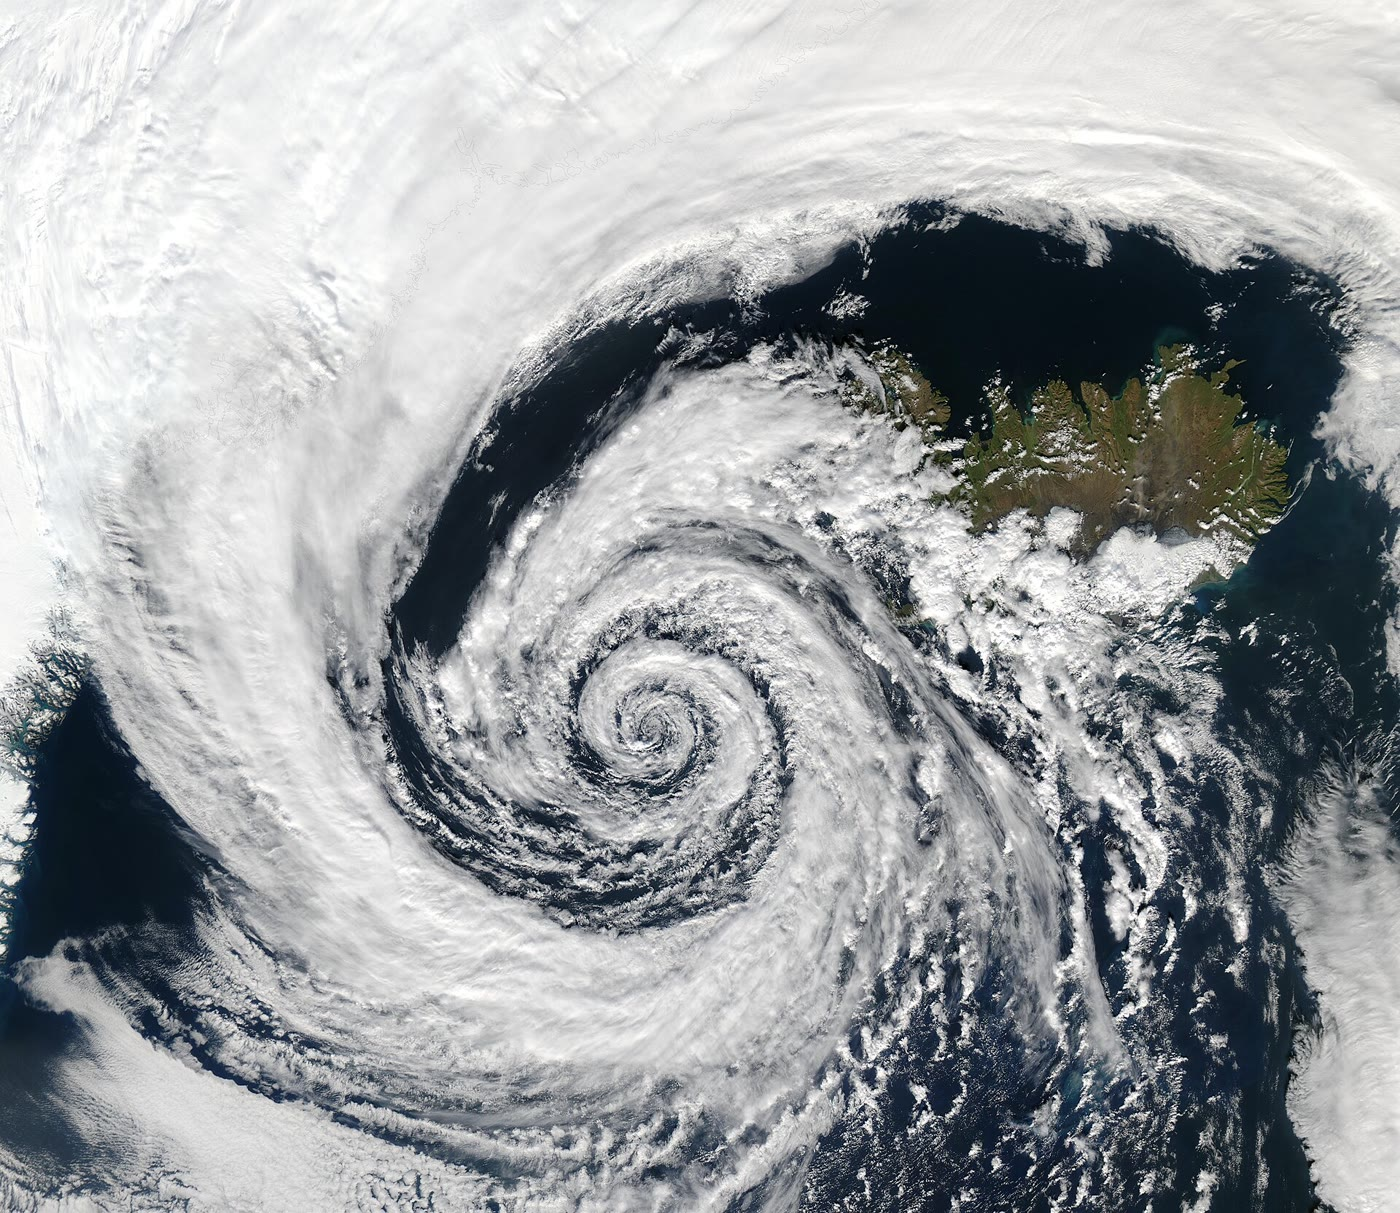
\includegraphics[width=\linewidth]{images/book1/g8-iceland-low.jpg}
\end{minipage}\hfill
\begin{minipage}[c]{0.6\linewidth}\raggedright
{\small A \omterm{def:g8:fronts-and-weather-maps:depression}{depression} south-west of Iceland (the island at the top right)
seen by NASA's Aqua satellite on 4~September 2003. Its \omterm{def:g4:clouds-rain-snow:cloud}{clouds} spiral
in towards the centre, turning anticlockwise as in every \omterm{def:g8:fronts-and-weather-maps:depression}{depression} of
the \omterm{def:g3:continents-and-oceans:equator}{northern hemisphere}. NASA/GSFC, MODIS Rapid Response Team, Jacques
Descloitres (public domain, via Wikimedia Commons).}
\end{minipage}
% ledger: commons:iceland-low, bom:highs-lows
\label{fig:g8:fronts-and-weather-maps:iceland}
\end{omfigure}

\section{Isobars and weather maps}

To see the \omterm{def:g8:fronts-and-weather-maps:depression}{depressions} and \omterm{def:g8:fronts-and-weather-maps:depression}{anticyclones}, forecasters draw \omterm{def:g2:drawing-to-map:map}{maps} of the
pressure. Every station measures its pressure and reduces it to \omterm{def:g4:world-physical-map:altitude}{sea level},
so that a station on a \omterm{def:g1:landscapes-around-us:landform}{mountain} can be compared with one on the \omterm{def:g1:landscapes-around-us:water}{coast}.
Then lines are drawn through all the places where the pressure is the
same.
% ledger: bom:isobars

\begin{definition}[Isobar]\label{def:g8:fronts-and-weather-maps:isobar}
An \emph{isobar}\index{isobar} is a line on a \omterm{def:g2:drawing-to-map:map}{map} joining places where
the pressure at \omterm{def:g4:world-physical-map:altitude}{sea level} is the same. Isobars are labelled in
hectopascals and are often drawn every \qty{4}{hPa}.
\end{definition}
% ledger: bom:isobars (the 4 hPa step is the one of this book's maps)

Around a \omterm{def:g8:fronts-and-weather-maps:depression}{depression} the \omterm{def:g8:fronts-and-weather-maps:isobar}{isobars} form closed loops, with the lowest
pressure at the centre, marked L; around an \omterm{def:g8:fronts-and-weather-maps:depression}{anticyclone} they form loops
with the highest pressure at the centre, marked H. Where the \omterm{def:g8:fronts-and-weather-maps:isobar}{isobars} are
close together, the pressure changes quickly from one place to the next,
and the wind is strong; where they are far apart, the wind is light.
% ledger: bom:isobars

\begin{omfigure}
\begin{tikzpicture}
\begin{axis}[width=14cm, axis equal image, xmin=0, xmax=2400, ymin=0, ymax=1600,
  hide axis, clip=true, axis background/.style={fill=white}]
  \addplot[isobar] table {figdata/out/grade-8-weather_map-isobars.dat};
  \addplot[warm front] table {figdata/out/grade-8-weather_map-warm.dat};
  \addplot[cold front] table {figdata/out/grade-8-weather_map-cold.dat};
  \addplot[quiver={u=\thisrow{u}, v=\thisrow{v}}, -{Stealth[length=1.5mm]}, omMeth, line width=0.6pt]
    table[x=x, y=y] {figdata/out/grade-8-weather_map-winds.dat};
  \addplot[only marks, mark=none, nodes near coords, point meta=explicit symbolic,
    every node near coord/.style={anchor=center, font=\tiny, fill=white, inner sep=0.6pt}]
    table[x=x, y=y, meta=level] {figdata/out/grade-8-weather_map-labels.dat};
  \node[font=\Large\bfseries, omCold, fill=white, inner sep=1pt] at (axis cs:690,1010) {L};
  \node[font=\scriptsize, anchor=north, fill=white, inner sep=0.5pt] at (axis cs:690,968) {980};
  \node[font=\Large\bfseries, omWarm] at (axis cs:1950,520) {H};
  \node[font=\scriptsize, anchor=north] at (axis cs:1950,485) {1034};
  \addplot[only marks, mark=square*, mark size=2pt, black] table[x=x, y=y] {figdata/out/grade-8-weather_map-town.dat};
  \node[font=\footnotesize\bfseries, anchor=west, fill=white, inner sep=1pt] at (axis cs:870,380) {T};
  \fill[white] (axis cs:1930,1450) rectangle (axis cs:2290,1585);
  \draw[line width=1pt] (axis cs:1950,1480) -- (axis cs:2250,1480);
  \pgfplotsinvokeforeach{1950,2050,2150,2250}{\draw (axis cs:#1,1460) -- (axis cs:#1,1500);}
  \node[font=\scriptsize, anchor=south] at (axis cs:2100,1495) {300 km};
\end{axis}
\end{tikzpicture}

{\small A \omterm{def:g1:watching-the-weather:weather}{weather} \omterm{def:g2:drawing-to-map:map}{map} of an imaginary day in the \omterm{def:g3:continents-and-oceans:equator}{northern hemisphere},
computed from a model of the pressure. \omterm{def:g8:fronts-and-weather-maps:isobar}{Isobars} every \qty{4}{hPa}; the
\omterm{def:g8:fronts-and-weather-maps:depression}{depression} L (\qty{980}{hPa}) carries a \omterm{def:g8:fronts-and-weather-maps:front}{warm front} (red) and a \omterm{def:g8:fronts-and-weather-maps:front}{cold front}
(blue); the \omterm{def:g8:fronts-and-weather-maps:depression}{anticyclone} H (\qty{1034}{hPa}) lies to the east. Green arrows:
the wind, longer where it is stronger. T: the town of the problem.}
% ledger: bom:isobars, bom:highs-lows, mo:fronts (figdata/grade-8/weather_map.py)
\label{fig:g8:fronts-and-weather-maps:map}
\end{omfigure}

\begin{method}[Reading a weather map]
\begin{enumerate}
  \item Find the centres: L for the \omterm{def:g8:fronts-and-weather-maps:depression}{depressions}, H for the \omterm{def:g8:fronts-and-weather-maps:depression}{anticyclones},
        with their pressures.
  \item Read the \omterm{def:g8:fronts-and-weather-maps:isobar}{isobars}: their values rise towards H and fall towards L.
        Close \omterm{def:g8:fronts-and-weather-maps:isobar}{isobars} mean a strong wind.
  \item Find the wind's direction: in the \omterm{def:g3:continents-and-oceans:equator}{northern hemisphere} it blows
        nearly along the \omterm{def:g8:fronts-and-weather-maps:isobar}{isobars}, with the low pressure on its left,
        turned a little towards the low.
  \item Find the \omterm{def:g8:fronts-and-weather-maps:front}{fronts} and the way they move (the side of their
        symbols), then the air on each side: what is coming next?
\end{enumerate}
\end{method}
% ledger: bom:isobars, bom:highs-lows, mo:fronts

\begin{example}[The weather at the town T]
On the \omterm{def:g2:drawing-to-map:map}{map}, T lies south of the \omterm{def:g8:fronts-and-weather-maps:front}{warm front} and east of the \omterm{def:g8:fronts-and-weather-maps:front}{cold front}: in
the warm air between the two \omterm{def:g8:fronts-and-weather-maps:front}{fronts}. The \omterm{def:g8:fronts-and-weather-maps:front}{warm front} has already passed
it. The \omterm{def:g8:fronts-and-weather-maps:isobar}{isobars} run from the south-west to the north-east there, with the
low to the north-west: the wind blows from the south-west, warm and damp.
The \omterm{def:g8:fronts-and-weather-maps:front}{cold front} is coming from the west. Its triangles point east,
towards the town: within hours there will be a short spell of heavy
showers and gusts, then the wind will turn to the west or north-west, the
air will get cooler and the sky will clear.
\end{example}
% ledger: ucar:cold-front (figdata/grade-8/weather_map.py: wind at T from 227 degrees)

A barometer gives its own warning, even without a \omterm{def:g2:drawing-to-map:map}{map}. Suppose the whole
\omterm{def:g2:drawing-to-map:map}{map} above drifted east, without changing, at \qty{40}{km} an hour, and a
recording barometer stood at a station S, east of the \omterm{def:g8:fronts-and-weather-maps:front}{fronts}. Over two and
a half days it would draw the record below.

\begin{omfigure}
\begin{tikzpicture}
\begin{axis}[width=0.86\linewidth, height=5.4cm, xmin=0, xmax=60, ymin=980, ymax=1040,
  xtick={0,12,...,60}, ytick={980,990,...,1040},
  xlabel={hours from the start of the record}, ylabel={pressure (hPa)},
  axis x line=bottom, axis y line=left, axis line style={-},
  grid=major, grid style={black!10},
  tick label style={font=\scriptsize}, label style={font=\small}, clip=false]
  \draw[omWarm!80!black, dashed] (axis cs:26.28,980) -- (axis cs:26.28,1040);
  \draw[omCold!80!black, dashed] (axis cs:38.49,980) -- (axis cs:38.49,1040);
  \node[font=\scriptsize, omWarm!80!black, anchor=south, fill=white, inner sep=1pt] at (axis cs:26.28,1032) {warm front};
  \node[font=\scriptsize, omCold!80!black, anchor=south, fill=white, inner sep=1pt] at (axis cs:38.49,1032) {cold front};
  \addplot[black!80, line width=1pt] table[x=hour, y=p_hPa] {figdata/out/grade-8-barogram-trace.dat};
  \node[font=\scriptsize, anchor=north west, align=left] at (axis cs:2,1028) {anticyclone:\\settled};
  \node[font=\scriptsize, anchor=west] at (axis cs:39.5,986) {lowest};
\end{axis}
\end{tikzpicture}

{\small The record of a barometer at the station S while the \omterm{def:g2:drawing-to-map:map}{map} above
drifts east at \qty{40}{km} an hour (an invented situation, computed from
the \omterm{def:g2:drawing-to-map:map}{map}'s pressure field). Dashed lines: the \omterm{def:g8:fronts-and-weather-maps:front}{warm front} and the \omterm{def:g8:fronts-and-weather-maps:front}{cold front}
passing the station.}
% ledger: (invented region: weather situation of figdata/grade-8/weather_map.py, record from figdata/grade-8/barogram.py)
\end{omfigure}

\begin{example}[Reading a barometer's record]\label{ex:g8:fronts-and-weather-maps:barogram}
For the first 8 hours the pressure rises to about \qty{1031}{hPa}: the
\omterm{def:g8:fronts-and-weather-maps:depression}{anticyclone} passes over S, with settled \omterm{def:g1:watching-the-weather:weather}{weather}. Then it falls for 30
hours, by about \qty{45}{hPa}: the \omterm{def:g8:fronts-and-weather-maps:depression}{depression} is coming. It falls fastest a few hours
before the \omterm{def:g8:fronts-and-weather-maps:front}{warm front} passes, more slowly in the warm air behind it,
and reaches its lowest, about \qty{986}{hPa}, just as the \omterm{def:g8:fronts-and-weather-maps:front}{cold front}
passes. Then it rises: the \omterm{def:g8:fronts-and-weather-maps:depression}{depression} is moving away, and the cooler,
clearer air behind the \omterm{def:g8:fronts-and-weather-maps:front}{cold front} arrives.
% ledger: (invented region: figdata/grade-8/barogram.py), bom:highs-lows
\end{example}

\section{How a forecast is made}

\begin{definition}[Weather forecast]\label{def:g8:fronts-and-weather-maps:forecast}
A \emph{weather forecast}\index{weather forecast} is a statement of the
\omterm{def:g1:watching-the-weather:weather}{weather} expected at a place over the coming hours or days, worked out
from observations of the atmosphere and from the laws of physics.
\end{definition}
% ledger: mo:how-forecasts

A forecast is made in three steps. First, \omterm{def:g1:watching-the-weather:weather}{weather} services around the
world make millions of observations every day: temperature, rainfall,
pressure, wind and humidity, measured at ground stations, at \omterm{def:g2:water-on-earth:ocean}{sea}, by
\omterm{def:g1:watching-the-weather:weather}{weather} balloons, by radar and from satellites. Then these observations
are fed into computer models: very powerful computers work out, step by
step, how the atmosphere will change from its present state. Finally,
forecasters read the results, compare them with what they know of their
region, and write the forecast.
% ledger: mo:how-forecasts

\begin{history}[The first public forecast]
In 1854 a naval officer, Robert FitzRoy, was put at the head of a new
\omterm{def:g1:watching-the-weather:weather}{weather} office in London. Every morning at 9~o'clock, stations around the
\omterm{def:g1:landscapes-around-us:water}{coasts} measured the \omterm{def:g1:watching-the-weather:weather}{weather} and sent their readings to London by the
telegraph, the newest invention of the day. In 1859 a terrible \omterm{def:g5:natural-hazards:storm}{storm}, the
\emph{Royal Charter} gale, sank many ships; FitzRoy then set up a service
of \omterm{def:g5:natural-hazards:storm}{storm} warnings for sailors, which began in February 1861. On
1~August 1861 he went further and published the first public \omterm{def:g8:fronts-and-weather-maps:forecast}{weather
forecast} in a newspaper, \emph{The Times}. His forecasts looked one or two
days ahead and were very general; they were the start of the forecasts we
read today.
\end{history}
% ledger: mo:fitzroy

Forecasts have become much better. Over the past decades, forecasters
have gained about one extra day of good forecast every ten years: a
forecast for four days ahead is now as good as a forecast for one day
ahead was thirty years ago. But the further ahead a forecast looks, the
less sure it is, because small errors in the starting observations
grow as the computer goes forward in time.
% ledger: bauer:day-per-decade, mo:accuracy

\begin{inthefield}[Watching a front arrive]
On a day when the forecast announces a \omterm{def:g8:fronts-and-weather-maps:front}{front}, look at the sky every few
hours and note the time, the \omterm{def:g4:clouds-rain-snow:cloud}{clouds}, the wind and the temperature. Before
a \omterm{def:g8:fronts-and-weather-maps:front}{warm front}, do high streaks of \omterm{def:g4:clouds-rain-snow:cloud-families}{cirrus} come first? When a \omterm{def:g8:fronts-and-weather-maps:front}{cold front}
passes, does the temperature drop and the wind change? Compare your notes
with the \omterm{def:g1:watching-the-weather:weather}{weather} \omterm{def:g2:drawing-to-map:map}{map} of the day.
\end{inthefield}

\section{Exercises}

\begin{exercise}[$\star$]\label{exo:g8:fronts-and-weather-maps:1}
Give the meaning of each pair of letters and say whether the \omterm{def:g8:fronts-and-weather-maps:air-mass}{air mass} is
warm or cold, damp or dry: (a) mT; (b) cP; (c) cT; (d) mP.
\end{exercise}

\begin{exercise}[$\star$]\label{exo:g8:fronts-and-weather-maps:2}
Match each sign of a \omterm{def:g1:watching-the-weather:weather}{weather} \omterm{def:g2:drawing-to-map:map}{map} with its meaning: a blue line with
triangles; a red line with half circles; a line joining places with the
same pressure; the letter H; the letter L.
\end{exercise}

\begin{exercise}[$\star$]\label{exo:g8:fronts-and-weather-maps:3}
True or false? Correct the false sentences. (a) \omterm{def:g8:fronts-and-weather-maps:depression}{Anticyclones} usually bring
settled \omterm{def:g1:watching-the-weather:weather}{weather}. (b) The \omterm{def:g4:clouds-rain-snow:cloud}{clouds} of a \omterm{def:g8:fronts-and-weather-maps:front}{warm front} arrive after the \omterm{def:g8:fronts-and-weather-maps:front}{front}.
(c) Close \omterm{def:g8:fronts-and-weather-maps:isobar}{isobars} mean a light wind. (d) Cold air is denser than warm
air.
\end{exercise}

\begin{exercise}[$\star$]\label{exo:g8:fronts-and-weather-maps:4}
On the \omterm{def:g1:watching-the-weather:weather}{weather} \omterm{def:g2:drawing-to-map:map}{map} of this chapter: (a) what is the pressure at the
centre of the \omterm{def:g8:fronts-and-weather-maps:depression}{depression}? (b) Of the \omterm{def:g8:fronts-and-weather-maps:depression}{anticyclone}? (c) How many
hectopascals separate two neighbouring \omterm{def:g8:fronts-and-weather-maps:isobar}{isobars}? (d) By how many
hectopascals does the pressure differ between the two centres?
\end{exercise}

\begin{exercise}[$\star\star$]\label{exo:g8:fronts-and-weather-maps:5}
Put these events in the order in which they happen when a \omterm{def:g8:fronts-and-weather-maps:front}{warm front}
approaches and passes: steady \omterm{def:g4:clouds-rain-snow:precipitation}{rain}; thin streaks of \omterm{def:g4:clouds-rain-snow:cloud-families}{cirrus}; a grey veil
of altostratus; warmer, damper air; the \omterm{def:g4:clouds-rain-snow:cloud}{clouds} come lower and thicker.
\end{exercise}

\begin{exercise}[$\star\star$]\label{exo:g8:fronts-and-weather-maps:6}
Explain why the \omterm{def:g4:clouds-rain-snow:cloud}{clouds} of a \omterm{def:g8:fronts-and-weather-maps:front}{cold front} are towering, while those of a
\omterm{def:g8:fronts-and-weather-maps:front}{warm front} are spread in layers. Use the words \emph{wedge},
\emph{steep}, \emph{gentle slope}.
\end{exercise}

\begin{exercise}[$\star\star$]\label{exo:g8:fronts-and-weather-maps:7}
On the \omterm{def:g1:watching-the-weather:weather}{weather} \omterm{def:g2:drawing-to-map:map}{map}: (a) where is the wind strongest, near L or near H?
How can you tell? (b) North of L, from which direction does the wind
blow? (c) South of H? (d) Does the wind turn clockwise or anticlockwise
around L?
\end{exercise}

\begin{exercise}[$\star\star$]\label{exo:g8:fronts-and-weather-maps:8}
A barometer in a town reads \qty{1016}{hPa} at 6:00, \qty{1009}{hPa} at
12:00 and \qty{1003}{hPa} at 18:00. (a) By how much does the pressure
fall in 12 hours? (b) What is coming towards the town, a \omterm{def:g8:fronts-and-weather-maps:depression}{depression} or an
\omterm{def:g8:fronts-and-weather-maps:depression}{anticyclone}? (c) What \omterm{def:g1:watching-the-weather:weather}{weather} can the town expect?
\end{exercise}

\begin{exercise}[$\star\star$]\label{exo:g8:fronts-and-weather-maps:9}
Air that has stayed for a week over the Sahara moves north over the
Mediterranean \omterm{def:g2:water-on-earth:ocean}{Sea}. (a) Name this \omterm{def:g8:fronts-and-weather-maps:air-mass}{air mass} with its two letters. (b) Is it
hot or cold, damp or dry, when it leaves? (c) What could change in its
character as it crosses the \omterm{def:g2:water-on-earth:ocean}{sea}?
\end{exercise}

\begin{exercise}[$\star\star$]\label{exo:g8:fronts-and-weather-maps:10}
A forecast for four days ahead is now as good as a forecast for one day
ahead was thirty years ago. (a) How many days of good forecast have been
gained in thirty years? (b) How many is that for each ten years? (c) If
the same progress went on, in how many years would a five-day forecast be
as good as today's one-day forecast?
\end{exercise}

\begin{exercise}[$\star\star\star$]\label{exo:g8:fronts-and-weather-maps:11}
On the \omterm{def:g1:watching-the-weather:weather}{weather} \omterm{def:g2:drawing-to-map:map}{map}, use the \omterm{def:g2:drawing-to-map:scale}{scale} bar. (a) About how many kilometres
separate the centre L from the centre H? (b) Near L, two neighbouring
\omterm{def:g8:fronts-and-weather-maps:isobar}{isobars} are about \qty{80}{km} apart. By how many hectopascals does the
pressure change over \qty{100}{km} there? (c) Near H, two neighbouring
\omterm{def:g8:fronts-and-weather-maps:isobar}{isobars} are about \qty{140}{km} apart. Same question. (d) Where is the
wind stronger? Do the arrows of the \omterm{def:g2:drawing-to-map:map}{map} agree?
\end{exercise}

\begin{exercise}[$\star\star\star$]\label{exo:g8:fronts-and-weather-maps:12}
A \omterm{def:g8:fronts-and-weather-maps:front}{cold front} lies \qty{300}{km} west of a town and moves east at
\qty{50}{km} per hour; a \omterm{def:g8:fronts-and-weather-maps:front}{warm front} lies \qty{200}{km} west of another
town and moves at half that speed. (a) Which \omterm{def:g8:fronts-and-weather-maps:front}{front} reaches its town
first, and how many hours earlier? (b) Describe the \omterm{def:g1:watching-the-weather:weather}{weather} each town
will see when its \omterm{def:g8:fronts-and-weather-maps:front}{front} passes. (c) Which town will be warmer once its
\omterm{def:g8:fronts-and-weather-maps:front}{front} has passed?
\end{exercise}

\section{Problem: Will the match be rained off?}

\begin{problem}[{Weekend problem --- a football match is planned for 15:00
in the town T of the weather map; the cold front is coming: its speed is
measured on two maps and the hour it reaches the town is forecast}]
\label{pb:g8:fronts-and-weather-maps:1}
% ledger: ucar:cold-front (figdata/grade-8/weather_map.py; the front's speed and the length of the showers are exercise data)
At 09:00 a young forecaster looks at the \omterm{def:g1:watching-the-weather:weather}{weather} \omterm{def:g2:drawing-to-map:map}{map} of this chapter, then at the \omterm{def:g2:drawing-to-map:map}{map}
below: it shows the \omterm{def:g8:fronts-and-weather-maps:front}{cold front} near the town at 06:00 and at 09:00, on a
grid of squares of \qty{20}{km}.

\begin{center}
\begin{tikzpicture}
\begin{axis}[width=11cm, axis equal image, xmin=0, xmax=600, ymin=0, ymax=400,
  xtick={0,100,...,600}, ytick={0,100,...,400}, minor tick num=4,
  grid=both, minor grid style={black!10}, major grid style={black!25},
  tick label style={font=\scriptsize}, xlabel={distance east (km)}, ylabel={distance north (km)},
  label style={font=\small}]
  \addplot[cold front, densely dashed, opacity=0.55] table[x expr=\thisrow{x}-363.2, y expr=\thisrow{y}-180] {figdata/out/grade-8-weather_map-seq-06.dat};
  \addplot[cold front] table[x expr=\thisrow{x}-363.2, y expr=\thisrow{y}-180] {figdata/out/grade-8-weather_map-seq-09.dat};
  \addplot[only marks, mark=square*, mark size=2.2pt, black] table[x expr=\thisrow{x}-363.2, y expr=\thisrow{y}-180] {figdata/out/grade-8-weather_map-town.dat};
  \node[font=\footnotesize\bfseries, anchor=south west, fill=white, inner sep=1pt] at (axis cs:485,205) {T};
  \node[font=\scriptsize, fill=white, inner sep=1pt] at (axis cs:140,360) {06:00};
  \node[font=\scriptsize, fill=white, inner sep=1pt] at (axis cs:262,360) {09:00};
\end{axis}
\end{tikzpicture}
\end{center}

\noindent\textbf{Part I --- Reading the map.}\par\nopagebreak
\begin{enumerate}[beginpenalty=10000]
  \item On the \omterm{def:g1:watching-the-weather:weather}{weather} \omterm{def:g2:drawing-to-map:map}{map} of the chapter, is the town in the warm air or
        in the cold air? Which \omterm{def:g8:fronts-and-weather-maps:front}{front} has already passed over it?
  \item From which direction does the wind blow at the town?
  \item Which way is the \omterm{def:g8:fronts-and-weather-maps:front}{cold front} moving? How can you tell from its
        symbols?
  \item What \omterm{def:g1:watching-the-weather:weather}{weather} will the \omterm{def:g8:fronts-and-weather-maps:front}{cold front} bring when it passes?
\end{enumerate}

\noindent\textbf{Part II --- The front's speed.}\par\nopagebreak
\begin{enumerate}[resume, beginpenalty=10000]
  \item On the \omterm{def:g2:drawing-to-map:map}{map} above, at the height of the town, how far east is the
        \omterm{def:g8:fronts-and-weather-maps:front}{front} at 06:00? At 09:00?
  \item How many kilometres has the \omterm{def:g8:fronts-and-weather-maps:front}{front} moved in these three hours?
  \item What is its speed, in kilometres per hour?
  \item At 09:00, how many kilometres separate the \omterm{def:g8:fronts-and-weather-maps:front}{front} from the town?
\end{enumerate}

\noindent\textbf{Part III --- The forecast.}\par\nopagebreak
\begin{enumerate}[resume, beginpenalty=10000]
  \item If the \omterm{def:g8:fronts-and-weather-maps:front}{front} keeps the same speed, how many hours will it need to
        reach the town?
  \item At what time will it reach the town?
  \item Suppose the heavy showers last about one hour after the \omterm{def:g8:fronts-and-weather-maps:front}{front}
        passes. Will it still be raining at 15:00?
  \item The \omterm{def:g8:fronts-and-weather-maps:front}{front} could slow down to \qty{30}{km} per hour. When would it
        reach the town then? Write the forecast for the match in one or
        two sentences, giving both possible hours.
\end{enumerate}
\end{problem}
